% REV00 Tue 20 Jul 2021 08:12:01 WIB
% START Tue 20 Jul 2021 08:12:01 WIB

\chapter{Duabelas}

% 11
\begin{figure}[htbp]
% h: here, where the figure appears in the text (use can always just use [h] )
% t: top,  top of the current page.
% b: bottom of the current page.
% p: page, top of the next available float space (sometimes end up being the end of the document).
\centerline{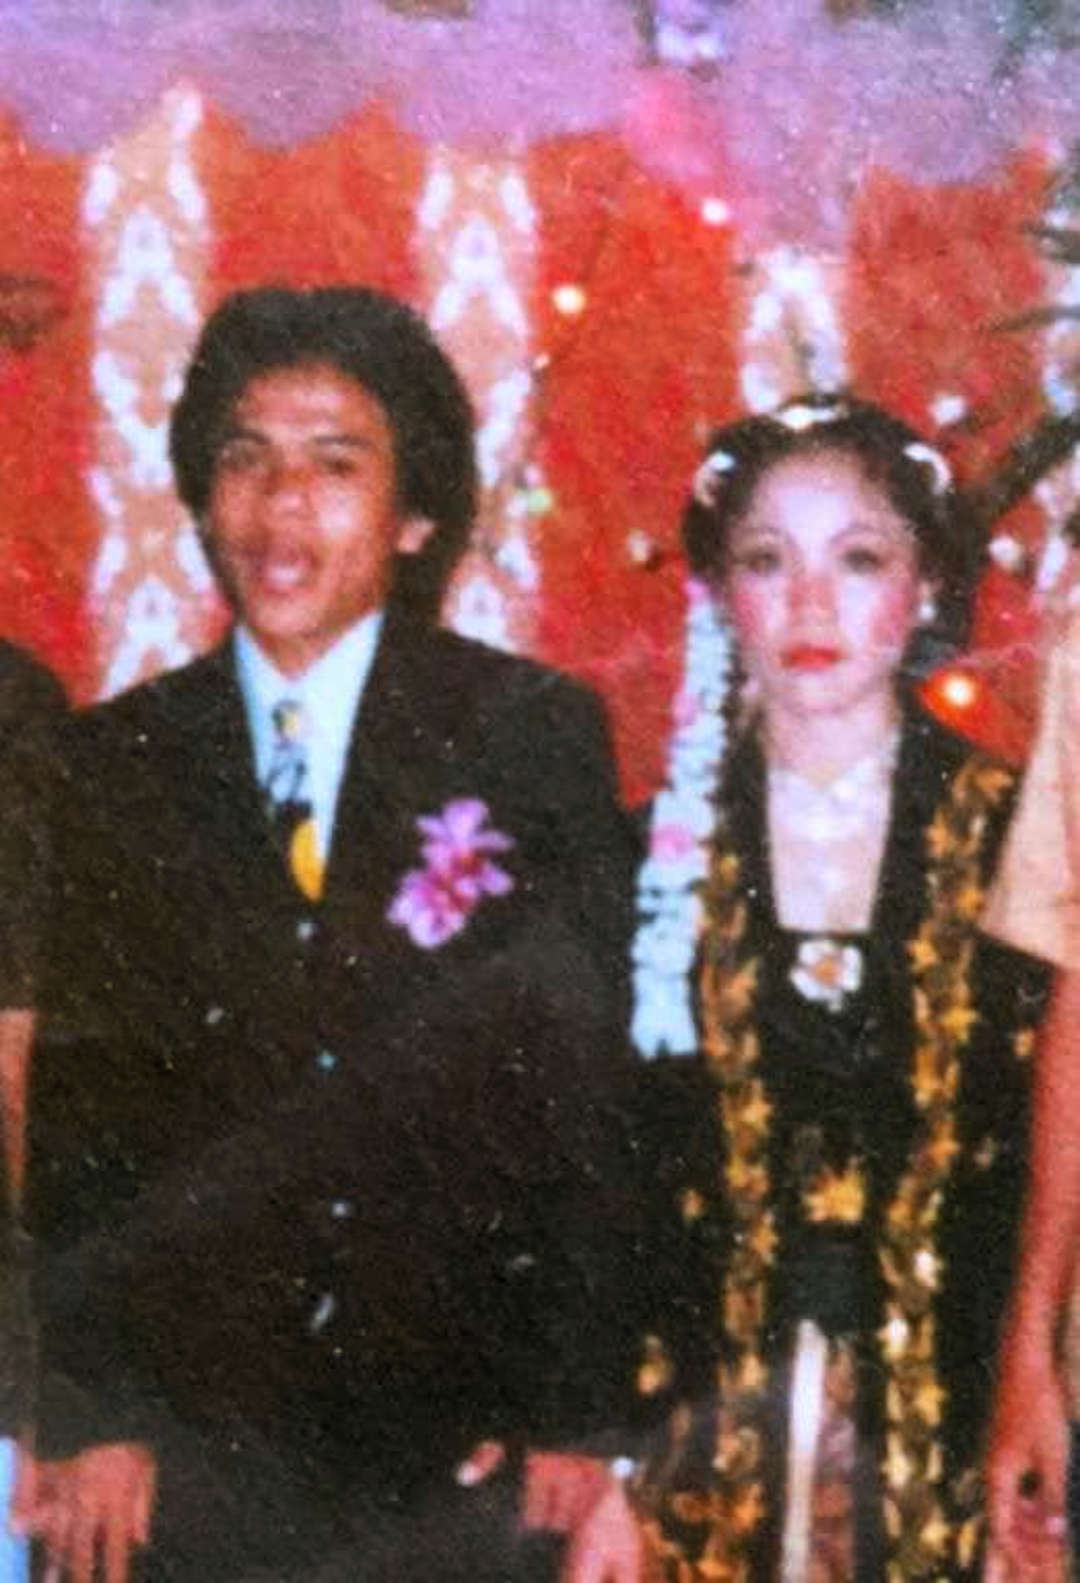
\includegraphics[scale=1.0]{01-12-01}}
\caption{"Album pernikahan Satiri-Fitria" Sumber: Koleksi Kelvy Safira dan Fitria Clara Zora}
\label{01-12-01}
\end{figure}
%

Puncak kebahagian baba, ibunda “ii”, istri tercinta Satiri, dan juga adik-adiknya adalah ketika akhirnya ia diwisuda. Jadi insinyur!

Itu adalah gelar yang ia pilih untuk dirinya. Koq bisa milih? Hingga pertengahan 80an, ijazah ITB memang hanya menuliskan kata “Sarjana”. Jadi, ya suka-sukamu lah…

Saat itu umumnya lulusan MIPA, termasuk Fisika, menggunakan gelar ‘Drs’ atau ‘Dra’; dan lulusan dari fakultas teknik memakai label ‘Ir’. Dan, waktu itu di ITB juga ada ijazah “Sarjana Muda”. Anda tahulah, kita itu mengadopsi konsep Londo: Doktorandus (artinya kandidat Doktor) dan Insinyur adalah S2.

Tetapi Satiri gagal berangkat ke Australia untuk melanjutkan studi pasca sarjana sebagai calon dosen UB. Ya, ia dinyatakan gagal!

Padahal, sebelum dia mangambil program UB saya mengatakan kepadanya bahwa dia sangat berbakat untuk menjadi dosen. Kita tahulah dia itu orang panggung, dan sesungguhnya kelas itu ya panggung juga.

Banyak fakta menunjukkan keberhasilan pendidikan lebih banyak dari guru yang menguasai pangggung kelas walaupun ia tidak sangat cerdas, jika dibandingkan dengan guru jenius tetapi sangat kaku di ruang kelas. Apalagi Satiri itu jenius. Anda bisa bayangkan betapa hebat murid-muridnya kelak.

Apa daya, cerita beralih ke jalan yang berbeda.

“Alhamdulillah…”, begitulah dia memeluk istrinya ketika dia kembali dari kantor pusat Schlumberger di Jakarta. Penandatanganan kontrak kerja. Pekerjaannya seperti apa, itu urusan nanti saja.

“Jadi juga kita jadi orang kayaaaaa…” teriaknya. Dalam hati.

Jauh hari kemudian saya baru memahami bahwa pekerjaan wireline, di Slb maupun di perusahaan sejenis lainnya, memang membutuhkan otak, tetapi juga otot. Lokasi pekerjaannya di sekitar lobang bor area yang diperkirakan mengandung minyak. Ya, kebanyakan hutan belantara atau bahkan di lepas pantai.

Pekerjaan dimulai dengan memanggul peralatan, menarik-narik kabel dan menyusun modul. Ketika modul siap terhubung dengan komputer dan ruang kendali, mereka disisipkan ke lubang bor.

Kalau itu sudah dimulai, maka pekerjaan tidak dapat dihentikan hingga dinilai selesai. Dan, itu bisa membutuhkan lima-hari-empat-malam. Pol harus tetap berjaga untuk setiap troble-shooting apapun.

Jangan harap ada bantuan. You are all on your own!

Bayarannya? Sehari kerja melebihi gaji bulanan seorang dosen. Sepadan kan? Mana ada orang pintar yang mau juga jadi kuli di hutan belantara. Set peralatan pun harganya jutaan dollar.

Tapi sebelum mampu melakukan pekerjaan spesifik seperti itu, tentu saja Satiri juga harus ikut pelatihan. Itu termasuk dasar ilmu kebumian dan perminyakan, elektronika dan instrumentasi, serta pemrosesan data. Di mana ia dikirim untuk mempelajari ilmu dasar itu?

Di pusat pelatihan Slb Perth, AUSTRALIA!

(Skenario mana saja hasilnya sama: Ke Australia!)

Bagaimana dengan statusnya yang sudah berkeluarga? Buat manajemen Slb, Satiri sudah menandatangani kontrak bahwa selama empat tahun pertama penempatan kerja di Slb tidak diperkenankan untuk berkeluarga.

Itu artinya empat tahun setelah training. Empat tahun untuk dijadikan kuli di lapangan minyak. Bahaya bawa perempuan ke lapangan kan? Itu cuma alasan perusahaan cerdas menggaet kuli cerdas.

Bagi perusahaan, yang penting semua ada di Kontrak.

Tidak sedikit kasus bahwa kertas menjadi jauh lebih penting dari fakta. Again, you have to take itu, or leave it!

***

Satiri selalu teringat pada pandangan penuh harap dari mata ibunda dan adik-adiknya kala ia berumur sebelas, berjibaku mencari dan menjual kembang, dengan naik sepeda di kolong batangan.

Dalam rongga batinnya, itulah dian yang tak akan pernah berhenti bercahaya.

Konon, Satiri meminta orang tuanya untuk memberi nama “Dian” pada adik bungsunya, yang lahir ketika dia di SMA. Anak Betawi koq namanya Dian? Hahaha… Mungkin ini tanda-tanda kemajuan.

Dalam penerbangan perdananya ke Perth, ia bermimpi bahwa ia akan dengan leluasa membiayai adik-adiknya sekolah, setinggi-tingginya.

Orang Betawi harus sekolah tinggi!

Benar saja, semua adik-adiknya akhirnya mampu untuk mengecap pendidikan tinggi. Satiri yang membiayai mereka. Dua di antaranya bahkan lulus dari Departemen Fisika ITB! Jadi, tiga dari enam anak baba-ibundanya yang hanya mengecap beberapa tahun sekolah rendah itu lulus dari perguruan ternama.

Salah seorang adiknya, Maing, bahkan menyelesaikan PhD dalam bidang teknik nuklir di ITB-nya di Jepang, Titech! Bang Maing bahkan sudah bekerja sekitar satu dekade ini buat Badan Tenaga Atom Internasioal (IAEA) yang bermarkas di Wina, dalam rangka menjaga perdamaian dunia dari senjata nuklir.

Ini mungkin yang katanya lompatan kuantum (quantum leap)!

***

Tidak salah jika Satiri memilih untuk segera menjadi orang kaya. Sebab, kemiskinan itu dapat menjauhkan orang dari Kebaikan. Tetapi kaya itu juga bukanlah banyak harta. Kaya adalah kekayaan jiwa. Artinya?

Artinya, di sepanjang hidupnya Satiri memilih untuk terutama membela keluarga. Begitu kan yang diinginkan Tuhan? Dimulai dari keluarga. Kalau bukan begitu, mengapa Satiri kecil bertanya tentang ‘minyak’, ‘elektronika’ dan ‘Australia’?

Apakah Satiri juga akan pergi ke Rusia, seperti yang juga ditanyakan pada gurunya yang kedua Pak Paijo?

Tuhan punya rencana yang mungkin agak berbeda. Lebih dari setahun ia harus mengikuti kontrak pelatihan di Australia. Sempat juga ia beberapa kali kembali ke Rawa Belong, melepas kangen yang membuncah untuk segera memeluk kembali istri dan ketiga anaknya. Ya, seorang putranya lahir sebelum ia berangkat ke Australia!

Kangennya belum lepas, ia dikirim kembali untuk pelatihan tingkat lanjutan di Montrouge, Perancis, dan kemudian juga di Parma, Italia.

Bukan ke Rusia. Di sana mungkin ada beruang merah yang menanti menerkamnya. Kita tentu tidak akan pernah tahu.

Dalam penempatan pertama, Satiri mendapat tugas di Port Harcourt, Nigeria. Itu sebelas jam jalan darat ke arah Selatan ibukota Abuja. Jauh betul itu dari Rawa Belong. Tidak apa-apa asal jadi orang kaya!

Itu arti dari sabar.

Belum setahun, mucul kembali adatnya seperti ketika menghadap Pak Lesilolo, sang Legenda gurunya yang ketiga, Kepala SMAN XI Jakarta, sekolahnya.

“Boss, bagaimana kalau saya membawa anak dan isteri saya?” Pintanya, tetapi tetap terdengar seperempat nada ditinggikan. Mengancam.

“You…” Cuma itu yang keluar dari mulut bosnya yang terdiam beberapa saat. Boss tahu betul bahwa pekerjaan Satiri selalu sangat memuaskan. Ia juga orang yang periang. Bahkan belakangan di Seluruh Schlumberger ia lebih dikenal sebagai “Crazy Satiri”.

Bagaimana tidak gila, dalam setiap pelatihan Satiri hampir selalu jadi juara pertama. Paling sial juara kedua. Teman-teman pelatihannya tahu betul bahwa Satiri tidak pernah belajar selain di ruang kelas.

Setiap malam selama semua pelatihan itu ia hanya menggoda teman-temannya. Keluyuran, ‘klacar-klucur’, keluar masuk café, menikmati berbagai hidangan yang tidak pernah ia temukan di Rawa Belong.

Yang teman-temannya tidak tahu adalah jam belajarnya di ruang kelas itu sudah jauh melebihi kuota belajarnya di ITB. Naah…

“Gua cuma kalah sama si Joaquin Schneider, Ren” katanya kepadaku suatu ketika. “Itu orang Jerman kutu buku, enggak gaul. Siang malam kerjanya belajar doang. Sering gua kerjain dah pas praktikum… Hahahah…”

Nah, sekarang boss mau bilang apa kalau Satiri mau bawa istri dan ketiga anak-anaknya?

“Could you guarantee that it will not come back to me?” (“Kamu bisa jamin itu tidak akan merepotkan saya?”)

“Yes. Definitely!” Jawaban standar, apapun akibatnya.

“Hell, do it. But remember, we never talk about this, right?” (“Terserah kamu. Anggap saja kita tidak pernah membicarakannya yah…”)

“Bodo amat. Emangnya gua pikirin,” sontak jawabnya dalam ekspresi Betawi. (“Hell, who care…”)

“You what?”

“Fcuk you!”jawabnya sambil kabur. Kuli-kuli Schlumberger membacanya sebagai “Yes, okay…”

Siapa yang enggak bisa gila jauh dari istri hampir setahun?
\\[10pt]

Sumber tulisan asli \url{https://www.facebook.com/reno.alamsyah.94/posts/10226581568111508}

